
\documentclass[fontsize=12pt]{scrartcl} % A4 paper and 12pt font size

\usepackage[T1]{fontenc} % Use 8-bit encoding that has 256 glyphs
%\usepackage{fourier} % Use the Adobe Utopia font for the document - comment this line to return to the LaTeX default
\usepackage{spverbatim}
\usepackage[bottom=6em]{geometry}
\usepackage[english]{babel} % English language/hyphenation
\usepackage[babel=true]{csquotes} 
\usepackage{amsmath,amsfonts,amsthm} % Math packages
\usepackage{lipsum} % Used for inserting dummy 'Lorem ipsum' text into the template
\usepackage{graphicx}
\usepackage{titlepic}
\usepackage{bbm}
\usepackage{color}
\usepackage{sectsty} % Allows customizing section commands
\usepackage{listings} %Allows Java code
\setlength{\headheight}{0pt} % Customize the height of the header


%\numberwithin{equation}{section} % Number equations within sections (i.e. 1.1, 1.2, 2.1, 2.2 instead of 1, 2, 3, 4)
%\numberwithin{figure}{section} % Number figures within sections (i.e. 1.1, 1.2, 2.1, 2.2 instead of 1, 2, 3, 4)
%\numberwithin{table}{section} % Number tables within sections (i.e. 1.1, 1.2, 2.1, 2.2 instead of 1, 2, 3, 4)


%----------------------------------------------------------------------------------------
%	TITLE SECTION
%----------------------------------------------------------------------------------------

\newcommand{\horrule}[1]{\rule{\linewidth}{#1}} % Create horizontal rule command with 1 argument of height
\title{	
 %  
\includegraphics[width=4cm]{lia-logo.jpg} % also works with logo.pdf
\normalfont \normalsize 
\textsc{Intelligent Agents, EPFL} \\ [20pt] % Your university, school and/or department name(s)
\horrule{0.5pt} \\[0.4cm] % Thin top horizontal rule
\huge Deliberative	 agents \\ % The assignment title
\horrule{2pt} \\[0.5cm] % Thick bottom horizontal rule
}
\author{Jeremy Gotteland \& Quentin Praz} % Your name
\date{\normalsize\today} % Today's date or a custom date
\begin{document}
\maketitle % Print the title

%----------------------------------------------------------------------------------------
%	PROBLEMS SECTION
%----------------------------------------------------------------------------------------

\section*{World representation}
\subsection*{State representation}
Recall that the agent here refers to a single vehicle.
We chose to represent the state of an agent as the following:
\begin{itemize}
\item Current city: The city in which the agent is currently located.

\item Vehicle: The type of vehicle

\item Cost: The cost from initial city to arrive in that state. Computed as the number of kilometers times the cost per kilometers of the vehicle.

\item Available tasks: The tasks the agent has not picked up yet  

\item Carried tasks: The tasks the agent is carrying and has to deliver.

\item currentWeight / freeWeight: The sum of the carried tasks.

\item List of actions: list of actions necessary to arrive at this state from initial state.
\end{itemize}

Our \textit{State} object contains a method called 'getNextStates()' that returns the states in which we can arrive from current state. We differentiate three cases:

\begin{enumerate}

\item Next step could be to \textbf{deliver} any of the task we currently carry. Then our next city would be one the task's delivery city. We would end up with one task less to carry and less weight.

\item Next step could be to \textbf{pickup} any of the task we yet have to pickup (available tasks) \textbf{given that we have enough free weight to carry that task}. Then our next city would be one of the available task's pickup city. We would end up with one more carried task, one available task less, and more weight.
\item Next step could be to \textbf{delivery and pickup} some tasks if the pickup and delivery cities are the same, given that the removal of the carried task gives us enough weight to pickup a new one. This is a mixture of the two previosu scenarios.

\end{enumerate}


\textbf{We are in a final state when we have no more available tasks to pickup, nor carried tasks to deliver}


\section*{Heuristic}

First, let's define the cost of going from a city to another one as the following (CPK being the Cost per Kilometer of the vehicle): 

$$ C(c_i, c_j) = D(c_i, c_j) * CPK $$


Our heuristic for A* is the following:

Given a state \textbf{S} in city $c_{current}$, that can go deliver tasks in a set of city \textbf{D}, and pickup tasks in a set of cities \textbf{P}, their union being the set of next possible cities given state \textbf{S} : $\textbf{N} = \textbf{D} \cup \textbf{P}$ the heuristic $H_S$ is equal to 

$$ H_S = \max(\max(C(c_{current}, c_n)), \max(C(x)) ), \forall c_n \in \textbf{N} $$


This heuristic makes sense because it does not overestimate the cost: in every case we will have to go through at least one of those paths, so we take the maximum of them all as our heuristic because it will be the minimum distance we will go through. \\ \\

It is optimal because the choices we make are directed towards taking the shortest paths to the final state where we will have delivered all possible tasks.



\section*{Performance Comparisons between BFS and A*}

We first ran the simulation with only one agent through both algorithms, as well as the naive algorithm, trying consecutive values for the number of tasks. \\
We observe that the performance of the BFS algorithm and the naive algorithm are quite close. \\ Moreover, when we try to compute BFS for more than 8 tasks, we get a Timeout exception from Logist. \\
A*, as an addition to being quicker, also gives better performance as for the total distance covered. 

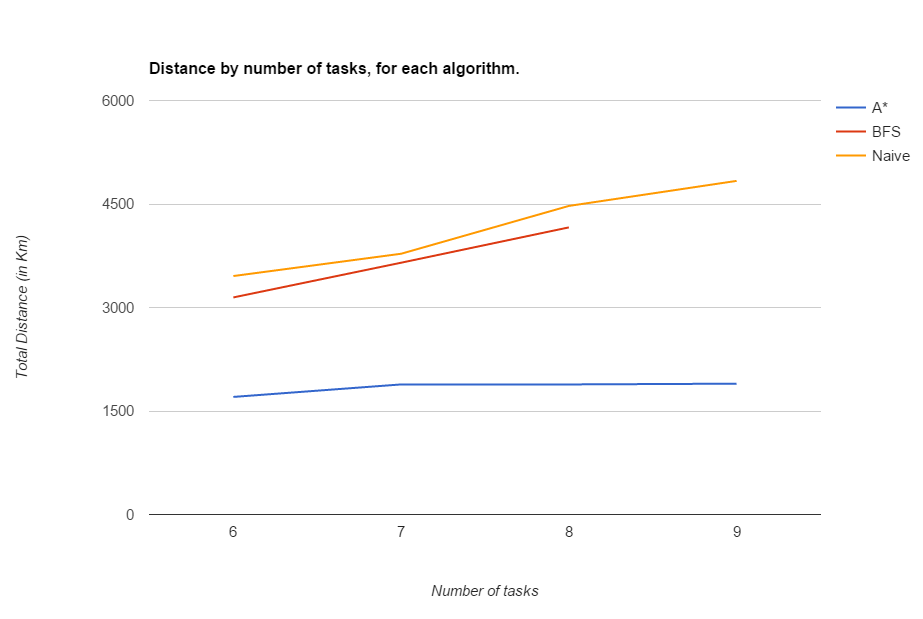
\includegraphics[width=.5\linewidth]{distance-nbtask.png}
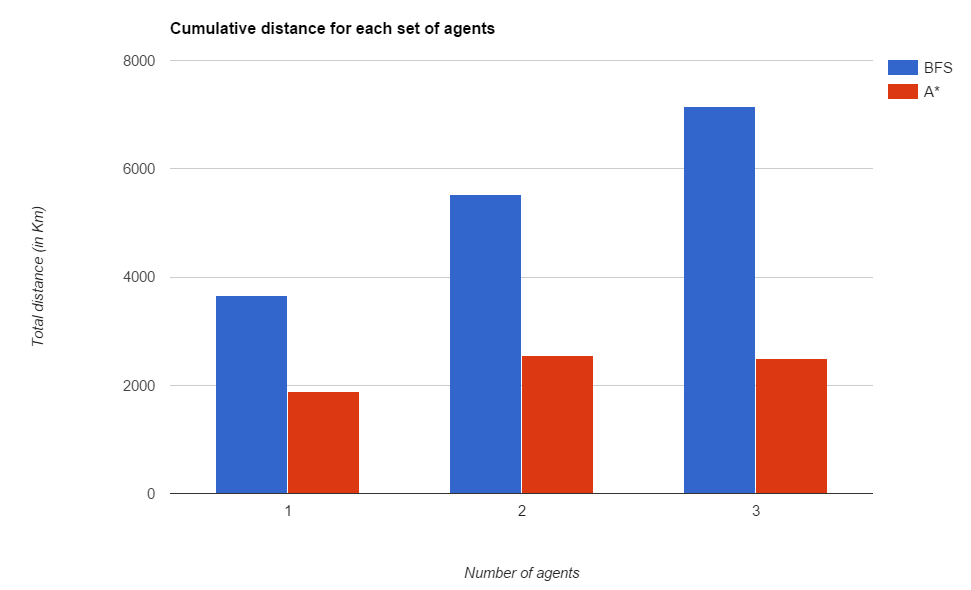
\includegraphics[width=.5\linewidth]{cumdist-nbagents.png} \\


Then we run the simulation with 1, 2, and 3 agents, for 7 tasks. \\
As discussed with the TAs, we discovered a bug in the Logist platform, which causes the first action from the agent's plan is \textbf{executed before the next agent starts to compute his plan}. Thus, the performance of the following agents is greatly improve as the problem they face is a subset of the initial problem (one less task), and so on for the next agents.. \\

None of those 2 algorithms is suited for cooperation as the agents do not consider each other. However, because of the problem previously stated, the A* algorithm gives very good results as the number of agents increases.



\section*{Conclusion}

In this exercice, we discovered two main algorithms for implementing deliberative agents: BFS and A*. 

We proved by observation that, if the heuristic is carefully chosen, A* outperforms BFS greatly as the number of tasks and agent increases. \\
This is due to the fact that the heuristic guides the algorithm towards the right direction, whereas BFS's performance is very dependent on the order in which we visit the neighbours of each node. \\ \\
Using DFS (Depth-first Search) with pruning instead of BFS would have given better performance

\end{document}          
